% Topic 3.5: Layer 2 Scaling Solutions [ADVANCED]
% Digital Finance Introduction
\documentclass[11pt,aspectratio=169]{beamer}
\usetheme{Madrid}

% ======================= PACKAGES =======================
\usepackage{graphicx}
\usepackage{booktabs}
\usepackage{adjustbox}
\usepackage{multicol}
\usepackage{amsmath}
\usepackage{amssymb}
\usepackage{tikz}
\usetikzlibrary{arrows,shapes,positioning,shadows,trees}
\usepackage{listings}
\usepackage{xcolor}

% ======================= COLOR DEFINITIONS =======================
% Primary color scheme: Blue/Teal for Digital Finance
\definecolor{dfblue}{RGB}{0,102,204}
\definecolor{dfteal}{RGB}{0,153,153}
\definecolor{dfcyan}{RGB}{51,187,204}
\definecolor{dflightblue}{RGB}{153,204,255}
\definecolor{dflightblue2}{RGB}{173,214,255}
\definecolor{dflightblue3}{RGB}{193,224,255}
\definecolor{dflightblue4}{RGB}{213,234,255}

% Accent colors for finance applications
\definecolor{dfgreen}{RGB}{44, 160, 44}
\definecolor{dfred}{RGB}{214, 39, 40}
\definecolor{dforange}{RGB}{255, 127, 14}
\definecolor{dfgray}{RGB}{127, 127, 127}

% Utility colors
\definecolor{lightgray}{RGB}{240, 240, 240}
\definecolor{midgray}{RGB}{180, 180, 180}
\definecolor{codebg}{RGB}{245, 245, 245}

% ======================= THEME CUSTOMIZATION =======================
% Apply Digital Finance color scheme to Madrid theme
\setbeamercolor{palette primary}{bg=dflightblue3,fg=dfblue}
\setbeamercolor{palette secondary}{bg=dflightblue2,fg=dfblue}
\setbeamercolor{palette tertiary}{bg=dfteal,fg=white}
\setbeamercolor{palette quaternary}{bg=dfblue,fg=white}

\setbeamercolor{structure}{fg=dfblue}
\setbeamercolor{section in toc}{fg=dfblue}
\setbeamercolor{subsection in toc}{fg=dfteal}
\setbeamercolor{title}{fg=dfblue}
\setbeamercolor{frametitle}{fg=dfblue,bg=dflightblue3}
\setbeamercolor{block title}{bg=dflightblue2,fg=dfblue}
\setbeamercolor{block body}{bg=dflightblue4,fg=black}

% Remove navigation symbols for cleaner look
\setbeamertemplate{navigation symbols}{}

% Clean itemize/enumerate
\setbeamertemplate{itemize items}[circle]
\setbeamertemplate{enumerate items}[default]

% Margins for readability
\setbeamersize{text margin left=8mm,text margin right=8mm}

% ======================= LISTINGS CONFIGURATION =======================
% Python code style
\lstdefinestyle{pythonstyle}{
    language=Python,
    basicstyle=\ttfamily\footnotesize,
    keywordstyle=\color{dfblue}\bfseries,
    stringstyle=\color{dforange},
    commentstyle=\color{dfgray}\itshape,
    numberstyle=\tiny\color{dfgray},
    numbers=left,
    numbersep=5pt,
    backgroundcolor=\color{codebg},
    showspaces=false,
    showstringspaces=false,
    showtabs=false,
    frame=single,
    rulecolor=\color{midgray},
    tabsize=4,
    captionpos=b,
    breaklines=true,
    breakatwhitespace=false,
    escapeinside={(*@}{@*)},
    xleftmargin=10pt,
    xrightmargin=10pt
}

% Solidity code style
\lstdefinestyle{soliditystyle}{
    language=Java, % closest approximation
    basicstyle=\ttfamily\footnotesize,
    keywordstyle=\color{dfteal}\bfseries,
    stringstyle=\color{dforange},
    commentstyle=\color{dfgray}\itshape,
    numberstyle=\tiny\color{dfgray},
    numbers=left,
    numbersep=5pt,
    backgroundcolor=\color{codebg},
    showspaces=false,
    showstringspaces=false,
    showtabs=false,
    frame=single,
    rulecolor=\color{midgray},
    tabsize=2,
    captionpos=b,
    breaklines=true,
    breakatwhitespace=false,
    escapeinside={(*@}{@*)},
    xleftmargin=10pt,
    xrightmargin=10pt,
    morekeywords={pragma, contract, function, returns, public, private, view, pure, payable, address, uint256, mapping, event, modifier}
}

% Inline code command
\newcommand{\code}[1]{\texttt{\color{dfblue}#1}}

% ======================= CUSTOM COMMANDS =======================
% Bottom annotation (Madrid-style)
\newcommand{\bottomnote}[1]{%
\vfill
\vspace{-2mm}
\textcolor{dflightblue2}{\rule{\textwidth}{0.4pt}}
\vspace{1mm}
\footnotesize
\textbf{#1}
}

% Compact list spacing
\newcommand{\compactlist}{%
\setlength{\itemsep}{0pt}%
\setlength{\parskip}{0pt}%
\setlength{\parsep}{0pt}%
}

% Chart placeholder
\newcommand{\chartplaceholder}[2][5cm]{%
\begin{center}
\begin{adjustbox}{max width=0.95\textwidth, max height=#1}
\framebox[\textwidth][c]{%
\rule{0pt}{#1}%
\textcolor{midgray}{[#2]}%
}
\end{adjustbox}
\end{center}
}

% ======================= FINANCE NOTATION MACROS =======================
% Probability and statistics
\newcommand{\E}{\mathbb{E}} % Expected value
\newcommand{\Var}{\mathrm{Var}} % Variance
\newcommand{\Cov}{\mathrm{Cov}} % Covariance
\newcommand{\Prob}{\mathbb{P}} % Probability

% Distributions
\newcommand{\Normal}{\mathcal{N}} % Normal distribution
\newcommand{\Uniform}{\mathcal{U}} % Uniform distribution

% Returns and prices
\newcommand{\Ret}{R} % Return
\newcommand{\LogRet}{r} % Log return
\newcommand{\Price}{S} % Price/Stock price
\newcommand{\Strike}{K} % Strike price

% Options and derivatives
\newcommand{\CallPrice}{C} % Call option price
\newcommand{\PutPrice}{P} % Put option price
\newcommand{\Greeks}[1]{\mathit{#1}} % Greek letters

% Risk measures
\newcommand{\VaR}{\mathrm{VaR}} % Value at Risk
\newcommand{\CVaR}{\mathrm{CVaR}} % Conditional VaR
\newcommand{\Sharpe}{\mathrm{SR}} % Sharpe Ratio

% Time series
\newcommand{\AR}{\mathrm{AR}} % Autoregressive
\newcommand{\MA}{\mathrm{MA}} % Moving average
\newcommand{\GARCH}{\mathrm{GARCH}} % GARCH

% Blockchain/Crypto
\newcommand{\Hash}{\mathrm{Hash}} % Hash function
\newcommand{\Block}{\mathcal{B}} % Block
\newcommand{\Chain}{\mathcal{C}} % Chain

% Real numbers, integers
\newcommand{\R}{\mathbb{R}}
\newcommand{\Z}{\mathbb{Z}}
\newcommand{\N}{\mathbb{N}}

% ======================= TIKZ STYLES =======================
% Styles for finance-related diagrams
\tikzstyle{process} = [rectangle, minimum width=3cm, minimum height=1cm, text centered, draw=dfblue, fill=dflightblue4, thick]
\tikzstyle{decision} = [diamond, minimum width=3cm, minimum height=1cm, text centered, draw=dfteal, fill=dflightblue4, thick]
\tikzstyle{arrow} = [thick,->,>=stealth,color=dfblue]
\tikzstyle{blockchain} = [rectangle, rounded corners, minimum width=2.5cm, minimum height=1cm, text centered, draw=dfteal, fill=dflightblue3, thick]
\tikzstyle{transaction} = [circle, minimum size=0.8cm, text centered, draw=dforange, fill=dflightblue4, thick]

% ======================= FOOTER TEMPLATE =======================
\setbeamertemplate{footline}{
    \hbox{\begin{beamercolorbox}[wd=\paperwidth,ht=2.5ex,dp=1ex,leftskip=.5em,rightskip=.5em]{author in head/foot}
    \tiny
    \textbf{Digital Finance} \hfill
    Joerg Osterrieder \hfill
    \insertdate \hfill
    Page \insertframenumber{} / \inserttotalframenumber
    \end{beamercolorbox}}
}

% ======================= SECTION DIVIDER TEMPLATE =======================
\AtBeginSection[]{
\begin{frame}[plain]
\vfill
\centering
\begin{beamercolorbox}[sep=12pt,center]{title}
\usebeamerfont{title}\LARGE\insertsection\par
\end{beamercolorbox}
\vfill
\end{frame}
}


% Additional TikZ libraries for L2 diagrams
\usetikzlibrary{chains,calc,decorations.pathreplacing,fit,backgrounds}

% Custom styles for L2 diagrams (from T3.2)
\tikzstyle{blocknode} = [rectangle, rounded corners, minimum width=3cm, minimum height=2cm, text centered, draw=dfteal, fill=dflightblue3, thick]
\tikzstyle{hashbox} = [rectangle, rounded corners, minimum width=2cm, minimum height=0.8cm, text centered, draw=dfteal, fill=dflightblue3, thick, font=\footnotesize]
\tikzstyle{databox} = [rectangle, minimum width=2.5cm, minimum height=0.6cm, text centered, draw=dfblue, fill=dflightblue4, thick, font=\footnotesize]
\tikzstyle{keybox} = [rectangle, rounded corners, minimum width=2cm, minimum height=0.6cm, text centered, draw=dforange, fill=dflightblue4, thick, font=\footnotesize]
\tikzstyle{walletbox} = [rectangle, rounded corners, minimum width=2.5cm, minimum height=1cm, text centered, draw=dfgreen, fill=dflightblue4, thick]
\tikzstyle{networknode} = [circle, draw=dfblue, fill=dflightblue4, minimum size=0.8cm, thick]
% Additional L2-specific styles
\tikzstyle{l1box} = [rectangle, rounded corners, minimum width=4cm, minimum height=1cm, text centered, draw=dfteal, fill=dflightblue2, thick]
\tikzstyle{l2box} = [rectangle, rounded corners, minimum width=4cm, minimum height=1cm, text centered, draw=dforange, fill=dforange!15, thick]
\tikzstyle{bridgebox} = [rectangle, rounded corners, minimum width=2cm, minimum height=0.8cm, text centered, draw=dfpurple, fill=dfpurple!15, thick]

\title[Topic 3.5: Layer 2 Scaling]{Topic 3.5: Layer 2 Scaling Solutions [ADVANCED]}
\subtitle{Scaling Ethereum and Beyond}
\author{Joerg Osterrieder}
\institute{Digital Finance}
\date{2025}

\begin{document}

% =======================================================================
% SLIDE 1: TITLE SLIDE
% =======================================================================
\begin{frame}[plain]
\titlepage
\end{frame}

% =======================================================================
% SLIDE 2: LEARNING OBJECTIVES
% =======================================================================
\begin{frame}{Learning Objectives}
\textbf{By the end of this topic, you will be able to:}

\begin{enumerate}
\item \textbf{Explain} why Layer 2 solutions are needed and how they relate to the blockchain trilemma
\vspace{2mm}
\item \textbf{Compare} different L2 approaches: payment channels, sidechains, and rollups
\vspace{2mm}
\item \textbf{Distinguish} between Optimistic Rollups and ZK-Rollups, including their tradeoffs
\vspace{2mm}
\item \textbf{Evaluate} the security assumptions and trust models of various L2 solutions
\vspace{2mm}
\item \textbf{Analyze} the role of bridges in cross-chain communication and their risks
\vspace{2mm}
\item \textbf{Apply} knowledge of L2 economics to real-world use case selection
\end{enumerate}

\vspace{3mm}
\begin{block}{Core Question}
How can we process thousands of transactions per second without sacrificing decentralization or security?
\end{block}
\end{frame}

% =======================================================================
% SLIDE 3: PREREQUISITES - TRILEMMA RECAP
% =======================================================================
\begin{frame}{Prerequisites: The Blockchain Trilemma (Recap from T3.2)}
\textbf{Every blockchain must balance three properties:}

\begin{center}
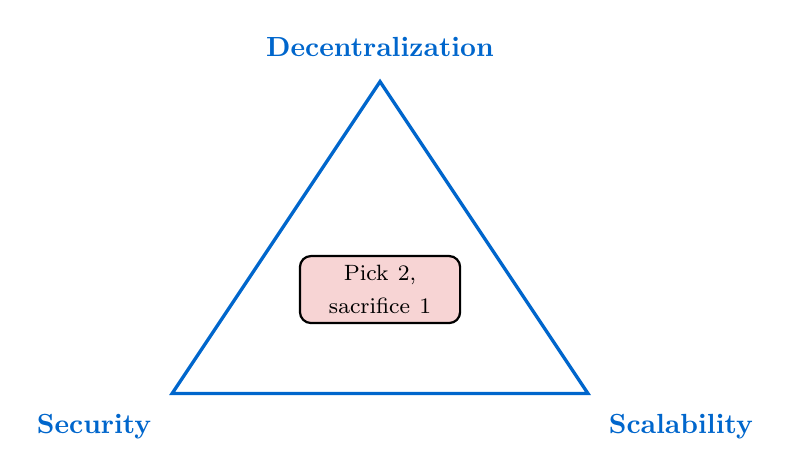
\begin{tikzpicture}[scale=1.1]
% Triangle
\coordinate (D) at (0, 2.8);
\coordinate (Se) at (-2.4, -0.8);
\coordinate (Sc) at (2.4, -0.8);

\draw[very thick, dfblue] (D) -- (Se) -- (Sc) -- cycle;

% Labels
\node[above=2mm of D, font=\bfseries, text=dfblue] {Decentralization};
\node[below left=2mm of Se, font=\bfseries, text=dfblue] {Security};
\node[below right=2mm of Sc, font=\bfseries, text=dfblue] {Scalability};

% Center impossible zone
\node[draw, thick, rounded corners, fill=dfred!20, minimum width=2cm, text width=1.8cm, align=center] at (0, 0.4) {
\footnotesize Pick 2,\\
sacrifice 1
};
\end{tikzpicture}
\end{center}

\vspace{3mm}
\textbf{The Problem:} Ethereum L1 processes $\sim$15 Transactions Per Second (TPS). Visa processes $\sim$24,000 TPS.

\textbf{The Question:} Can we scale without centralizing?

\bottomnote{Layer 2 solutions aim to break this trilemma by building \textit{on top} of secure L1s}
\end{frame}

% =======================================================================
% SLIDE 4: PREREQUISITES - GAS FEES
% =======================================================================
\begin{frame}{Prerequisites: The Gas Fee Problem}
\textbf{Why are Ethereum transactions expensive?}

\begin{columns}[T]
\begin{column}{0.48\textwidth}
\textbf{Block Space is Scarce}
\begin{itemize}\compactlist
\item Each block has limited capacity
\item Users bid for inclusion (gas fees)
\item High demand = high fees
\item 2021 peak: \$50+ for simple transfers
\end{itemize}

\vspace{3mm}
\textbf{The User Experience Problem}
\begin{itemize}\compactlist
\item Small transactions become uneconomical
\item \$5 coffee + \$20 fee = unusable
\item Prices out retail users
\item Benefits only whales
\end{itemize}
\end{column}
\begin{column}{0.48\textwidth}
\begin{center}
\textbf{Transaction Throughput Comparison}

\vspace{3mm}
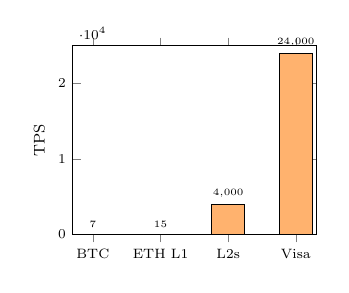
\begin{tikzpicture}[scale=0.7]
\begin{axis}[
    width=6cm, height=5cm,
    ybar,
    ylabel={\footnotesize TPS},
    ylabel style={font=\footnotesize},
    symbolic x coords={BTC, ETH L1, L2s, Visa},
    xtick=data,
    xticklabel style={font=\scriptsize},
    yticklabel style={font=\scriptsize},
    ymin=0, ymax=25000,
    bar width=0.6cm,
    nodes near coords,
    nodes near coords style={font=\tiny},
    every node near coord/.append style={anchor=south},
]
\addplot[fill=dforange!60] coordinates {(BTC, 7) (ETH L1, 15) (L2s, 4000) (Visa, 24000)};
\end{axis}
\end{tikzpicture}
\end{center}
\end{column}
\end{columns}

\vspace{3mm}
\begin{block}{Key Insight}
Layer 2 solutions process transactions off-chain, then settle on L1 -- getting L2 speed with L1 security.
\end{block}
\end{frame}

% =======================================================================
% SLIDE 5: WHAT IS LAYER 2?
% =======================================================================
\begin{frame}{What Is Layer 2?}
\begin{block}{Definition}
\textbf{Layer 2 (L2)} refers to any off-chain network, system, or technology built on top of a blockchain (Layer 1) to extend its capabilities -- primarily scaling and speed -- while inheriting the security of the underlying L1.
\end{block}

\vspace{3mm}
\begin{center}
\begin{tikzpicture}[scale=0.9]
% L2 layer
\node[l2box, minimum width=10cm, minimum height=1.2cm] (l2) at (0,2) {
\textbf{Layer 2:} Fast, cheap transactions
};

% Bridge
\draw[very thick, dfpurple, <->] (0,1.2) -- (0,0.3) node[midway, right, font=\footnotesize] {Periodic settlement};

% L1 layer
\node[l1box, minimum width=10cm, minimum height=1.2cm] (l1) at (0,-0.5) {
\textbf{Layer 1 (Ethereum):} Secure, decentralized, slow
};

% Annotations
\node[right=0.5cm of l2, text width=3cm, font=\scriptsize] {2,000-4,000+ TPS\\Low fees (\$0.01-0.10)};
\node[right=0.5cm of l1, text width=3cm, font=\scriptsize] {15-30 TPS\\Higher fees (\$1-50+)};
\end{tikzpicture}
\end{center}

\vspace{3mm}
\textbf{Analogy:} L2 is like a bar tab -- you make many small transactions throughout the night, but only settle once at the end.
\end{frame}

% =======================================================================
% SLIDE 6: WHY L2 MATTERS
% =======================================================================
\begin{frame}{Why Layer 2 Matters: The Scalability Crisis}
\begin{columns}[T]
\begin{column}{0.55\textwidth}
\textbf{The Problem (2020-2021)}
\begin{itemize}\compactlist
\item DeFi and NFT boom overwhelmed Ethereum
\item Gas fees spiked to \$50-200 per transaction
\item Small users priced out entirely
\item ``Ethereum is for whales only''
\end{itemize}

\vspace{3mm}
\textbf{The Stakes}
\begin{itemize}\compactlist
\item Mass adoption impossible at 15 TPS
\item Competitors (Solana, Avalanche) gaining ground
\item Ethereum risked losing its lead
\item Urgent need for scaling solutions
\end{itemize}
\end{column}
\begin{column}{0.42\textwidth}
\begin{center}
\fbox{\parbox{0.95\textwidth}{
\textbf{Scale Requirements:}\\[2mm]
\footnotesize
Current: 15-30 TPS\\
For global payments: 100,000+ TPS\\[2mm]
\textbf{Gap: 3,000x improvement needed}
}}
\end{center}

\vspace{3mm}
\textbf{L2 Solution Benefits:}
\begin{itemize}\compactlist
\item 90\%+ fee reduction
\item 100x+ throughput increase
\item Inherit L1 security
\item No L1 changes required
\end{itemize}
\end{column}
\end{columns}

\vspace{3mm}
\bottomnote{Vitalik Buterin: ``Rollups are the only viable scaling solution for Ethereum in the medium term''}
\end{frame}

% =======================================================================
% SLIDE 7: PAYMENT CHANNELS - CONCEPT
% =======================================================================
\begin{frame}{Payment Channels: The Original L2}
\begin{block}{Definition}
A \textbf{payment channel} is a two-party agreement to transact off-chain, with only the opening and closing transactions recorded on-chain.
\end{block}

\vspace{3mm}
\begin{center}
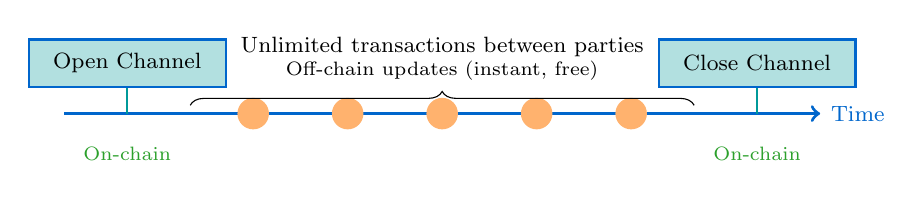
\begin{tikzpicture}[scale=0.8]
% Timeline
\draw[very thick, dfblue, ->] (0,0) -- (12,0) node[right] {\footnotesize Time};

% On-chain events
\node[databox, fill=dfteal!30] (open) at (1,0.8) {\footnotesize Open Channel};
\node[databox, fill=dfteal!30] (close) at (11,0.8) {\footnotesize Close Channel};

\draw[thick, dfteal] (1,0) -- (1,0.4);
\draw[thick, dfteal] (11,0) -- (11,0.4);

% Off-chain transactions
\foreach \x in {3,4.5,6,7.5,9} {
    \node[circle, fill=dforange!60, minimum size=0.4cm] at (\x, 0) {};
}
\node[above=0.3cm, font=\scriptsize] at (6,0) {Off-chain updates (instant, free)};

% Braces
\draw[decorate, decoration={brace, amplitude=5pt, raise=3pt}] (2,0) -- (10,0);
\node[above=0.6cm, font=\footnotesize] at (6,0) {Unlimited transactions between parties};

% Labels
\node[below=0.3cm, font=\scriptsize, text=dfgreen] at (1,0) {On-chain};
\node[below=0.3cm, font=\scriptsize, text=dfgreen] at (11,0) {On-chain};
\end{tikzpicture}
\end{center}

\vspace{3mm}
\textbf{Bar Tab Analogy:}
\begin{enumerate}\compactlist
\item \textbf{Open tab:} Lock funds in a shared account (on-chain)
\item \textbf{Buy drinks:} Update balance off-chain (instant, no fees)
\item \textbf{Close tab:} Settle final balance on-chain
\end{enumerate}
\end{frame}

% =======================================================================
% SLIDE 8: LIGHTNING NETWORK
% =======================================================================
\begin{frame}{Lightning Network: Bitcoin's Payment Channels}
\begin{columns}[T]
\begin{column}{0.55\textwidth}
\textbf{How It Works}
\begin{enumerate}\compactlist
\item Alice and Bob open a channel (on-chain)
\item They can transact unlimited times (off-chain)
\item Either party can close the channel anytime
\item Final balances settle on Bitcoin
\end{enumerate}

\vspace{3mm}
\textbf{Network of Channels}
\begin{itemize}\compactlist
\item Channels can be routed through intermediaries
\item Alice $\rightarrow$ Carol $\rightarrow$ Bob
\item No direct channel needed
\item Atomic: all-or-nothing routing
\end{itemize}

\vspace{3mm}
\textbf{Stats (2024):}
\begin{itemize}\compactlist
\item 15,000+ nodes
\item 60,000+ channels
\item \$200M+ capacity
\end{itemize}
\end{column}
\begin{column}{0.42\textwidth}
\begin{center}
\textbf{Lightning Network Topology}

\vspace{3mm}
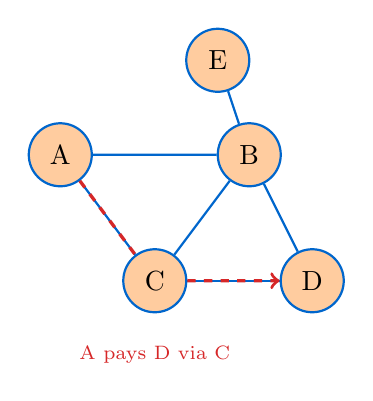
\begin{tikzpicture}[scale=0.8]
% Nodes
\node[networknode, fill=dforange!40] (a) at (0,2) {A};
\node[networknode, fill=dforange!40] (b) at (3,2) {B};
\node[networknode, fill=dforange!40] (c) at (1.5,0) {C};
\node[networknode, fill=dforange!40] (d) at (4,0) {D};
\node[networknode, fill=dforange!40] (e) at (2.5,3.5) {E};

% Channels
\draw[thick, dfblue] (a) -- (b);
\draw[thick, dfblue] (a) -- (c);
\draw[thick, dfblue] (b) -- (c);
\draw[thick, dfblue] (b) -- (d);
\draw[thick, dfblue] (b) -- (e);
\draw[thick, dfblue] (c) -- (d);

% Routing example
\draw[very thick, dfred, dashed, ->] (a) -- (c) -- (d);
\node[below=0.3cm of c, font=\scriptsize, text=dfred] {A pays D via C};
\end{tikzpicture}
\end{center}

\vspace{3mm}
\fbox{\parbox{0.9\textwidth}{\centering
\footnotesize \textbf{Limitation:} Only for payments, not smart contracts
}}
\end{column}
\end{columns}
\end{frame}

% =======================================================================
% SLIDE 9: SIDECHAINS - POLYGON
% =======================================================================
\begin{frame}{Sidechains: The Polygon Approach}
\begin{block}{Definition}
A \textbf{sidechain} is an independent blockchain that runs parallel to a main chain, connected via a two-way bridge. Sidechains have their own consensus and security.
\end{block}

\vspace{3mm}
\begin{center}
\begin{tikzpicture}[scale=0.85]
% Ethereum
\node[l1box, minimum width=5cm] (eth) at (0,0) {\textbf{Ethereum (L1)}};

% Bridge
\node[bridgebox, minimum width=2cm] (bridge) at (0,1.5) {Bridge};

% Polygon
\node[l2box, minimum width=5cm, fill=dfpurple!20, draw=dfpurple] (poly) at (0,3) {\textbf{Polygon PoS (Sidechain)}};

% Connections
\draw[very thick, dfpurple, <->] (eth) -- (bridge);
\draw[very thick, dfpurple, <->] (bridge) -- (poly);

% Annotations
\node[right=0.5cm of eth, text width=4cm, font=\scriptsize] {Secure, decentralized\\15-30 TPS};
\node[right=0.5cm of poly, text width=4cm, font=\scriptsize] {Own validators\\7,000+ TPS\\Own security model};
\end{tikzpicture}
\end{center}

\vspace{3mm}
\textbf{Key Difference from True L2:} Sidechains have \textit{independent security} -- they don't inherit Ethereum's security. If Polygon's validators collude, funds could be at risk.
\end{frame}

% =======================================================================
% SLIDE 10: SIDECHAIN TRUST MODEL
% =======================================================================
\begin{frame}{Sidechain Trust Model}
\begin{columns}[T]
\begin{column}{0.48\textwidth}
\textbf{Advantages}
\begin{itemize}\compactlist
\item \textcolor{dfgreen}{Very high throughput}
\item \textcolor{dfgreen}{Low fees (\$0.001-0.01)}
\item \textcolor{dfgreen}{EVM compatible (see Topic 3.4)}
\item \textcolor{dfgreen}{Easy to use}
\item \textcolor{dfgreen}{Mature ecosystem}
\end{itemize}

\vspace{3mm}
\textbf{Polygon PoS Stats:}
\begin{itemize}\compactlist
\item 100+ validators
\item 7,000+ TPS capacity
\item \$1B+ TVL
\item Used by: Uniswap, Aave, OpenSea
\end{itemize}
\end{column}
\begin{column}{0.48\textwidth}
\textbf{Disadvantages}
\begin{itemize}\compactlist
\item \textcolor{dfred}{Weaker security than L1}
\item \textcolor{dfred}{Fewer validators}
\item \textcolor{dfred}{Must trust validator set}
\item \textcolor{dfred}{Bridge risk}
\item \textcolor{dfred}{Not ``true'' L2}
\end{itemize}

\vspace{3mm}
\begin{center}
\fbox{\parbox{0.9\textwidth}{
\textbf{Security Model:}\\[2mm]
\footnotesize
Ethereum: 500,000+ validators\\
Polygon PoS: $\sim$100 validators\\[2mm]
\textcolor{dfred}{Smaller validator set = easier to attack}
}}
\end{center}
\end{column}
\end{columns}

\vspace{3mm}
\bottomnote{Sidechains trade security for speed -- acceptable for some use cases, not others}
\end{frame}

% =======================================================================
% SLIDE 11: PLASMA - HISTORICAL CONTEXT
% =======================================================================
\begin{frame}{Plasma: Historical Context}
\begin{columns}[T]
\begin{column}{0.55\textwidth}
\textbf{What Was Plasma? (2017)}
\begin{itemize}\compactlist
\item Proposed by Vitalik Buterin and Joseph Poon
\item Child chains anchored to Ethereum
\item Only submit state roots to L1
\item Users can exit to L1 if problems arise
\end{itemize}

\vspace{3mm}
\textbf{The Promise}
\begin{itemize}\compactlist
\item ``Millions of transactions per second''
\item Inherit Ethereum security
\item Low fees
\end{itemize}

\vspace{3mm}
\textbf{Why It Didn't Work}
\begin{itemize}\compactlist
\item \textcolor{dfred}{Complex exit game} (up to 2 weeks)
\item \textcolor{dfred}{Data availability problem}
\item \textcolor{dfred}{Hard to support smart contracts (general computation)}
\item \textcolor{dfred}{Mass exit vulnerability}
\end{itemize}
\end{column}
\begin{column}{0.42\textwidth}
\begin{center}
\textbf{Plasma Exit Game}

\vspace{3mm}
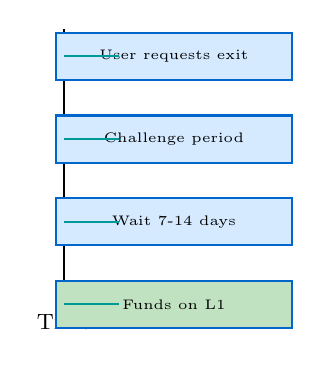
\begin{tikzpicture}[scale=0.7]
% Timeline
\draw[thick, ->] (0,0) -- (0,-5) node[below] {\footnotesize Time};

% Events
\node[databox, minimum width=3cm, font=\tiny] (exit) at (2,-0.5) {User requests exit};
\node[databox, minimum width=3cm, font=\tiny] (challenge) at (2,-2) {Challenge period};
\node[databox, minimum width=3cm, font=\tiny] (wait) at (2,-3.5) {Wait 7-14 days};
\node[databox, minimum width=3cm, fill=dfgreen!30, font=\tiny] (done) at (2,-5) {Funds on L1};

\draw[thick, dfteal] (0,-0.5) -- (1,-0.5);
\draw[thick, dfteal] (0,-2) -- (1,-2);
\draw[thick, dfteal] (0,-3.5) -- (1,-3.5);
\draw[thick, dfteal] (0,-5) -- (1,-5);
\end{tikzpicture}

\vspace{3mm}
\footnotesize \textcolor{dfred}{Too slow, too complex}
\end{center}
\end{column}
\end{columns}

\bottomnote{Plasma's limitations led directly to the development of rollups}
\end{frame}

% =======================================================================
% SLIDE 12: PLASMA LESSONS
% =======================================================================
\begin{frame}{Lessons from Plasma}
\textbf{Why Plasma Failed -- and What We Learned}

\begin{center}
\begin{tabular}{l|l|l}
\toprule
\textbf{Plasma Problem} & \textbf{Why It Matters} & \textbf{Rollup Solution} \\
\midrule
Data unavailability & Can't verify state & Post data to L1 \\
Complex exits & Bad UX & Simpler withdrawal process \\
Limited computation & Can't run smart contracts & EVM equivalence (see T3.4) \\
Mass exit attacks & Network congestion & Better exit mechanisms \\
\bottomrule
\end{tabular}
\end{center}

\vspace{5mm}
\begin{block}{The Key Insight}
Plasma tried to minimize data posted to L1. Rollups take the opposite approach: post all transaction data to L1, but execute it off-chain. This is called \textbf{data availability}.
\end{block}

\vspace{3mm}
\textbf{Result:} Rollups became the dominant L2 paradigm by 2021-2022.
\end{frame}

% =======================================================================
% SLIDE 13: ROLLUPS OVERVIEW
% =======================================================================
\begin{frame}{Rollups: The Modern L2 Approach}
\begin{block}{Definition}
A \textbf{rollup} executes transactions off-chain, then posts compressed transaction data and a state root to L1. Users can always reconstruct the L2 state from L1 data alone.
\end{block}

\vspace{3mm}
\begin{center}
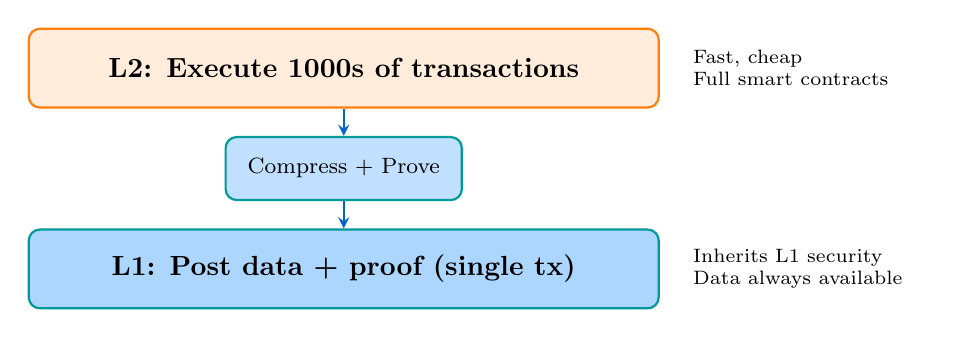
\begin{tikzpicture}[scale=0.85]
% L2 transactions
\node[l2box, minimum width=8cm] (batch) at (0,3) {
\textbf{L2: Execute 1000s of transactions}
};

% Compression
\node[hashbox, minimum width=3cm] (compress) at (0,1.5) {Compress + Prove};

% L1 posting
\node[l1box, minimum width=8cm] (l1) at (0,0) {
\textbf{L1: Post data + proof (single tx)}
};

% Arrows
\draw[arrow] (batch) -- (compress);
\draw[arrow] (compress) -- (l1);

% Annotations
\node[right=0.3cm of batch, font=\scriptsize, text width=3cm] {Fast, cheap\\Full smart contracts};
\node[right=0.3cm of l1, font=\scriptsize, text width=3cm] {Inherits L1 security\\Data always available};
\end{tikzpicture}
\end{center}

\vspace{3mm}
\textbf{Shipping Container Analogy:} Instead of shipping items one by one, pack 1,000 items into one container and ship that. More efficient, same destination.
\end{frame}

% =======================================================================
% SLIDE 14: DATA AVAILABILITY
% =======================================================================
\begin{frame}{The Data Availability Guarantee}
\textbf{Why posting data to L1 matters:}

\begin{columns}[T]
\begin{column}{0.55\textwidth}
\textbf{With Data Availability}
\begin{itemize}\compactlist
\item Anyone can reconstruct L2 state
\item No need to trust the sequencer
\item If L2 operators disappear, users can exit
\item ``Trustless'' scaling
\end{itemize}

\vspace{3mm}
\textbf{Without Data Availability}
\begin{itemize}\compactlist
\item Must trust operators to provide data
\item If operators withhold data, funds stuck
\item ``Trusted'' scaling (weaker security)
\item This was Plasma's problem
\end{itemize}
\end{column}
\begin{column}{0.42\textwidth}
\begin{center}
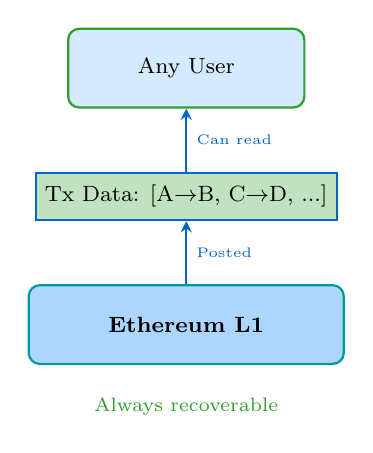
\begin{tikzpicture}[scale=0.8]
% Data on L1
\node[l1box, minimum width=4cm] (l1) at (0,0) {\footnotesize \textbf{Ethereum L1}};

% Data
\node[databox, above=0.8cm of l1, minimum width=3.5cm, fill=dfgreen!30] (data) {
\footnotesize Tx Data: [A$\rightarrow$B, C$\rightarrow$D, ...]
};

% User
\node[walletbox, above=0.8cm of data, minimum width=3cm] (user) {\footnotesize Any User};

% Arrows
\draw[arrow] (l1) -- (data) node[midway, right, font=\tiny] {Posted};
\draw[arrow] (data) -- (user) node[midway, right, font=\tiny] {Can read};

% Label
\node[below=0.3cm of l1, font=\scriptsize, text=dfgreen] {Always recoverable};
\end{tikzpicture}
\end{center}

\vspace{3mm}
\fbox{\parbox{0.9\textwidth}{\centering
\footnotesize \textbf{Key Property:}\\
Rollup security = L1 security\\
(assuming data is on L1)
}}
\end{column}
\end{columns}
\end{frame}

% =======================================================================
% SLIDE 15: OPTIMISTIC ROLLUPS - INTRO
% =======================================================================
\begin{frame}{Optimistic Rollups: Assume Valid, Prove Fraud}
\begin{block}{Definition}
\textbf{Optimistic Rollups} assume transactions are valid by default (``optimistic'') and only compute proofs if someone challenges a transaction during a dispute period.
\end{block}

\vspace{3mm}
\begin{center}
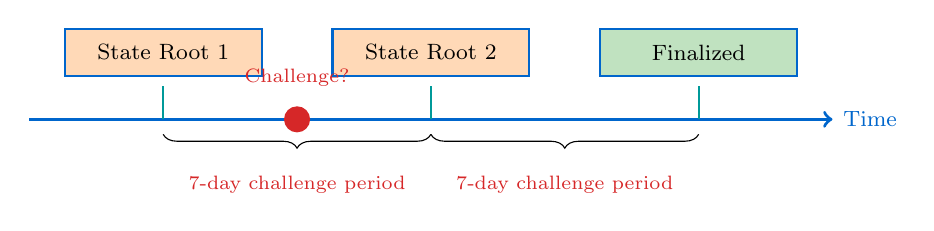
\begin{tikzpicture}[scale=0.85]
% Timeline
\draw[very thick, dfblue, ->] (0,0) -- (12,0) node[right] {\footnotesize Time};

% State roots
\node[databox, fill=dforange!30] (s1) at (2,1) {\footnotesize State Root 1};
\node[databox, fill=dforange!30] (s2) at (6,1) {\footnotesize State Root 2};
\node[databox, fill=dfgreen!30] (s3) at (10,1) {\footnotesize Finalized};

\draw[thick, dfteal] (2,0) -- (2,0.5);
\draw[thick, dfteal] (6,0) -- (6,0.5);
\draw[thick, dfteal] (10,0) -- (10,0.5);

% Challenge period
\draw[decorate, decoration={brace, amplitude=5pt, raise=3pt, mirror}] (2,-0.1) -- (6,-0.1);
\node[below=0.6cm, font=\scriptsize, text=dfred] at (4,0) {7-day challenge period};

\draw[decorate, decoration={brace, amplitude=5pt, raise=3pt, mirror}] (6,-0.1) -- (10,-0.1);
\node[below=0.6cm, font=\scriptsize, text=dfred] at (8,0) {7-day challenge period};

% Challenge
\node[circle, fill=dfred, minimum size=0.3cm] at (4,0) {};
\node[above=0.3cm, font=\scriptsize, text=dfred] at (4,0) {Challenge?};
\end{tikzpicture}
\end{center}

\vspace{3mm}
\textbf{How it works:}
\begin{enumerate}\compactlist
\item Sequencer posts state root to L1 (assumes valid)
\item Anyone can challenge with a \textbf{fraud proof} if they detect cheating
\item After 7 days with no successful challenge, state is finalized
\end{enumerate}

\vspace{2mm}
\textit{Analogy:} Like a warranty period where anyone can point out defects before the product is final.
\end{frame}

% =======================================================================
% SLIDE 16: FRAUD PROOFS EXPLAINED
% =======================================================================
\begin{frame}{Fraud Proofs: Keeping Optimistic Rollups Honest}
\begin{columns}[T]
\begin{column}{0.55\textwidth}
\textbf{The Fraud Proof Process}
\begin{enumerate}\compactlist
\item Sequencer posts: ``State changed from A to B''
\item Challenger says: ``That's wrong!''
\item Interactive dispute on L1:
    \begin{itemize}\compactlist
    \item Narrow down to single instruction
    \item L1 executes that instruction
    \item Whoever was wrong loses bond
    \end{itemize}
\end{enumerate}

\vspace{3mm}
\textbf{Why 7 Days?}
\begin{itemize}\compactlist
\item Gives everyone time to detect fraud
\item Allows time to submit challenge
\item Allows time to complete the dispute game
\item Works even during network congestion
\item \textit{Note: This delay exists to give anyone time to challenge potentially fraudulent transactions}
\end{itemize}
\end{column}
\begin{column}{0.42\textwidth}
\begin{center}
\textbf{Fraud Proof Timeline}

\vspace{3mm}
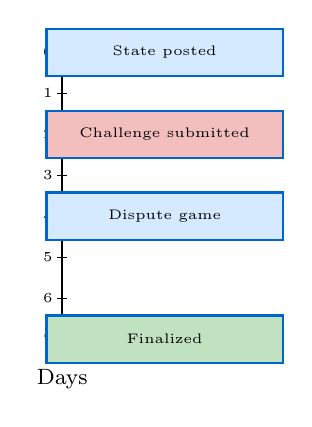
\begin{tikzpicture}[scale=0.65]
% Timeline
\draw[thick, ->] (0,0) -- (0,-6) node[below] {\footnotesize Days};

% Days
\foreach \y in {0,1,2,3,4,5,6,7} {
    \node[left, font=\tiny] at (0,-\y*0.8) {\y};
    \draw[thin] (-0.1,-\y*0.8) -- (0.1,-\y*0.8);
}

% Events
\node[databox, minimum width=3cm, font=\tiny] at (2,0) {State posted};
\node[databox, minimum width=3cm, font=\tiny, fill=dfred!30] at (2,-1.6) {Challenge submitted};
\node[databox, minimum width=3cm, font=\tiny] at (2,-3.2) {Dispute game};
\node[databox, minimum width=3cm, font=\tiny, fill=dfgreen!30] at (2,-5.6) {Finalized};
\end{tikzpicture}
\end{center}
\end{column}
\end{columns}

\bottomnote{In practice, fraud is rare because cheaters lose their bond -- it's not profitable}
\end{frame}

% =======================================================================
% SLIDE 17: OPTIMISM AND ARBITRUM
% =======================================================================
\begin{frame}{Optimism and Arbitrum: The Leading Optimistic Rollups}
\begin{columns}[T]
\begin{column}{0.48\textwidth}
\textbf{Optimism}
\begin{itemize}\compactlist
\item Launched 2021
\item EVM equivalent (see T3.4)
\item Simple fraud proof design
\item OP token for governance
\item ``Superchain'' vision
\item TVL: \$800M+ (2024)
\end{itemize}

\vspace{3mm}
\textbf{Notable Users:}
\begin{itemize}\compactlist
\item Uniswap
\item Aave
\item Synthetix
\end{itemize}
\end{column}
\begin{column}{0.48\textwidth}
\textbf{Arbitrum}
\begin{itemize}\compactlist
\item Launched 2021
\item EVM equivalent (see T3.4)
\item More complex fraud proofs
\item ARB token for governance
\item Arbitrum One + Nova
\item TVL: \$2.5B+ (2024)
\end{itemize}

\vspace{3mm}
\textbf{Notable Users:}
\begin{itemize}\compactlist
\item GMX
\item Radiant
\item Treasure
\end{itemize}
\end{column}
\end{columns}

\vspace{3mm}
\begin{center}
\fbox{\parbox{0.85\textwidth}{\centering
\textbf{Both offer:} 90\%+ fee reduction, 10-50x throughput increase, same Ethereum security (after 7 days)
}}
\end{center}
\end{frame}

% =======================================================================
% SLIDE 18: ZK-ROLLUPS - INTRO
% =======================================================================
\begin{frame}{ZK-Rollups: Prove Validity Mathematically}
\begin{block}{Simple Hook}
Imagine proving you know a secret without revealing the secret itself -- that's the power of zero-knowledge proofs.
\end{block}

\begin{block}{Definition}
\textbf{ZK-Rollups} use zero-knowledge proofs to cryptographically prove that all transactions in a batch are valid. No challenge period needed -- validity is mathematically guaranteed.
\end{block}

\vspace{2mm}
\textit{Analogy:} Like a math teacher verifying your homework is correct without checking every step.

\vspace{3mm}
\begin{center}
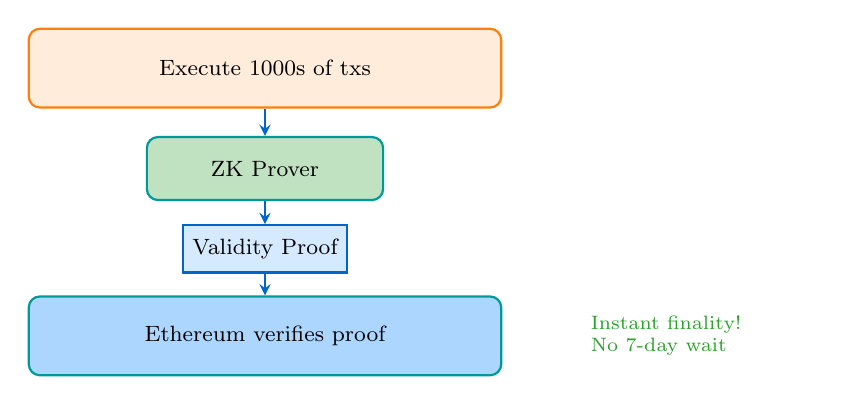
\begin{tikzpicture}[scale=0.85]
% L2 transactions
\node[l2box, minimum width=6cm] (batch) at (0,2.5) {\footnotesize Execute 1000s of txs};

% ZK Prover
\node[hashbox, minimum width=3cm, fill=dfgreen!30] (prover) at (0,1) {\footnotesize ZK Prover};

% Proof
\node[databox, minimum width=2cm] (proof) at (0,-0.2) {\footnotesize Validity Proof};

% L1
\node[l1box, minimum width=6cm] (l1) at (0,-1.5) {\footnotesize Ethereum verifies proof};

% Arrows
\draw[arrow] (batch) -- (prover);
\draw[arrow] (prover) -- (proof);
\draw[arrow] (proof) -- (l1);

% Instant finality
\node[right=1cm of l1, text width=3cm, font=\scriptsize, text=dfgreen] {Instant finality!\\No 7-day wait};
\end{tikzpicture}
\end{center}

\vspace{3mm}
\textbf{Key Difference from Optimistic:} Validity is proven \textit{before} posting, not after. This enables instant withdrawals to L1.
\end{frame}

% =======================================================================
% SLIDE 19: VALIDITY PROOFS EXPLAINED
% =======================================================================
\begin{frame}{Validity Proofs: How ZK-Rollups Work}
\begin{columns}[T]
\begin{column}{0.55\textwidth}
\textbf{Zero-Knowledge Proofs}
\begin{itemize}\compactlist
\item Prove a statement is true without revealing details
\item Example: ``I know the password'' without showing it
\item In ZK-rollups: ``These 1000 txs are valid'' in one small proof
\end{itemize}

\vspace{3mm}
\textbf{The Process}
\begin{enumerate}\compactlist
\item Sequencer executes transactions off-chain
\item ZK prover generates validity proof
\item Proof + state root posted to L1
\item L1 contract verifies proof (cheap!)
\item If proof valid, state is immediately finalized
\end{enumerate}

\vspace{2mm}
\textit{Analogy:} Like a math teacher checking your work upfront vs trusting you did it correctly.

\vspace{2mm}
\textbf{Proof Types:}
\begin{itemize}\compactlist
\item \textbf{SNARKs} (Succinct Non-interactive ARgument of Knowledge): smaller proofs, but need a ``trusted setup''
\item \textbf{STARKs} (Scalable Transparent ARgument of Knowledge): larger proofs, but don't require trusted setup
\item \textit{Technical names for two types of mathematical proof systems}
\end{itemize}
\end{column}
\begin{column}{0.42\textwidth}
\begin{center}
\fbox{\parbox{0.95\textwidth}{
\textbf{Proof Compression:}\\[2mm]
\footnotesize
1000 transactions\\
$\downarrow$\\
1 proof ($\sim$300 bytes)\\[2mm]
Verification: $\sim$500k gas\\
(cheaper than 1000 txs!)
}}
\end{center}

\vspace{3mm}
\textbf{Analogy:}\\[2mm]
\footnotesize
A teacher checking 1000 homework assignments vs. having a machine that instantly verifies ``all 1000 are correct'' in one step.
\end{column}
\end{columns}

\bottomnote{ZK proofs are computationally expensive to generate but cheap to verify}
\end{frame}

% =======================================================================
% SLIDE 20: ZKSYNC AND STARKNET
% =======================================================================
\begin{frame}{zkSync and StarkNet: The Leading ZK-Rollups}
\begin{columns}[T]
\begin{column}{0.48\textwidth}
\textbf{zkSync Era}
\begin{itemize}\compactlist
\item By Matter Labs
\item Launched 2023
\item EVM compatible (zkEVM, see T3.4)
\item SNARKs-based proofs (Succinct Non-interactive ARguments of Knowledge)
\item ZK token airdrop 2024
\item TVL: \$150M+ (2024)
\end{itemize}

\vspace{3mm}
\textbf{Key Features:}
\begin{itemize}\compactlist
\item Native account abstraction
\item Hyperchain vision
\item Growing ecosystem
\end{itemize}
\end{column}
\begin{column}{0.48\textwidth}
\textbf{StarkNet}
\begin{itemize}\compactlist
\item By StarkWare
\item Launched 2022
\item Custom language (Cairo)
\item STARKs-based proofs (Scalable Transparent ARguments of Knowledge)
\item STRK token 2024
\item TVL: \$200M+ (2024)
\end{itemize}

\vspace{3mm}
\textbf{Key Features:}
\begin{itemize}\compactlist
\item No trusted setup
\item StarkEx for app chains
\item Strong research team
\end{itemize}
\end{column}
\end{columns}

\vspace{3mm}
\begin{block}{The EVM Compatibility Challenge}
Making ZK proofs for EVM execution is extremely difficult. zkSync achieved it with zkEVM; StarkNet uses a custom VM (requires learning Cairo).
\end{block}
\end{frame}

% =======================================================================
% SLIDE 21: OPTIMISTIC VS ZK COMPARISON
% =======================================================================
\begin{frame}{Optimistic vs. ZK Rollups: Head-to-Head}
\begin{center}
\begin{tabular}{l|c|c}
\toprule
\textbf{Aspect} & \textbf{Optimistic Rollups} & \textbf{ZK-Rollups} \\
\midrule
Withdrawal time & \textcolor{dfred}{7 days*} & \textcolor{dfgreen}{Minutes} \\
Proof type & Fraud proof (if challenged) & Validity proof (always) \\
Computation cost & \textcolor{dfgreen}{Minimal} & \textcolor{dfred}{Heavy (prover)} \\
EVM compatibility & \textcolor{dfgreen}{High (mature)} & \textcolor{dfred}{Developing} \\
Security model & Optimistic + challenge & Cryptographic \\
Maturity & \textcolor{dfgreen}{More mature} & \textcolor{dfred}{Newer} \\
Examples & Optimism, Arbitrum & zkSync, StarkNet \\
\bottomrule
\end{tabular}

\vspace{2mm}
{\scriptsize *This delay exists to give anyone time to challenge potentially fraudulent transactions}
\end{center}

\vspace{5mm}
\begin{columns}[T]
\begin{column}{0.48\textwidth}
\textbf{Choose Optimistic when:}
\begin{itemize}\compactlist
\item Need full EVM compatibility
\item 7-day withdrawal acceptable
\item Deploying existing contracts
\end{itemize}
\end{column}
\begin{column}{0.48\textwidth}
\textbf{Choose ZK when:}
\begin{itemize}\compactlist
\item Need fast withdrawals
\item High-security applications
\item Future-proofing matters
\end{itemize}
\end{column}
\end{columns}
\end{frame}

% =======================================================================
% SLIDE 22: TRADEOFF DEEP DIVE
% =======================================================================
\begin{frame}{Rollup Tradeoffs: A Deeper Look}
\begin{center}
\begin{tikzpicture}[scale=0.9]
% Axes
\draw[very thick, ->] (0,0) -- (8,0) node[right] {\footnotesize Throughput};
\draw[very thick, ->] (0,0) -- (0,5) node[above] {\footnotesize Security/Finality};

% Quadrants
\node[l2box, minimum width=2.5cm, minimum height=1.5cm] (op) at (5,1.5) {
\footnotesize \textbf{Optimistic}\\
\tiny High TPS, 7d wait
};

\node[l2box, minimum width=2.5cm, minimum height=1.5cm, fill=dfgreen!20] (zk) at (3,4) {
\footnotesize \textbf{ZK}\\
\tiny Lower TPS, instant
};

\node[l1box, minimum width=2cm, minimum height=1cm] (l1) at (1,3) {
\footnotesize \textbf{L1}\\
\tiny Most secure
};

\node[process, minimum width=2cm, minimum height=1cm, fill=dfpurple!20] (side) at (6.5,3.5) {
\footnotesize \textbf{Sidechain}\\
\tiny Fastest, less secure
};

% Legend
\node[below=0.5cm of op, font=\scriptsize] {Current sweet spot};
\node[above right=0.1cm and 0.5cm of zk, font=\scriptsize, text=dfgreen] {Future direction};
\end{tikzpicture}
\end{center}

\vspace{3mm}
\textbf{Industry consensus (2024):} ZK-rollups are the long-term future, but optimistic rollups are more practical today due to EVM maturity. Both will likely coexist.
\end{frame}

% =======================================================================
% SLIDE 23: BRIDGES - CROSS-CHAIN
% =======================================================================
\begin{frame}{Bridges: Connecting L1 and L2}
\begin{block}{Definition}
A \textbf{bridge} is a protocol that allows assets to move between different blockchains or layers. Bridges lock assets on one chain and mint equivalent assets on another.
\end{block}

\vspace{3mm}
\begin{center}
\begin{tikzpicture}[scale=0.85]
% L1
\node[l1box, minimum width=3cm] (l1) at (0,0) {\footnotesize Ethereum};
\node[databox, above=0.5cm of l1, font=\tiny] (lock) {ETH locked};

% Bridge
\node[bridgebox, minimum width=2cm] (bridge) at (4,0) {\footnotesize Bridge Contract};

% L2
\node[l2box, minimum width=3cm] (l2) at (8,0) {\footnotesize Arbitrum};
\node[databox, above=0.5cm of l2, font=\tiny] (mint) {aETH minted};

% Arrows
\draw[very thick, dfblue, ->] (l1) -- node[above, font=\tiny] {Deposit} (bridge);
\draw[very thick, dfblue, ->] (bridge) -- node[above, font=\tiny] {Mint} (l2);
\draw[very thick, dfred, ->] (l2) to[bend left=30] node[below, font=\tiny] {Withdraw} (l1);
\end{tikzpicture}
\end{center}

\vspace{3mm}
\textbf{Bridge Types:}
\begin{itemize}\compactlist
\item \textbf{Native/Canonical:} Official rollup bridges (most secure, slowest)
\item \textbf{Third-party:} Hop, Across, Stargate (faster, more risk)
\item \textbf{CEX bridges:} Via exchanges (convenient, custodial)
\end{itemize}
\end{frame}

% =======================================================================
% SLIDE 24: BRIDGE SECURITY RISKS
% =======================================================================
\begin{frame}{Bridge Security: The Weak Link}
\textbf{Bridges are prime targets for hackers:}

\begin{center}
\begin{tabular}{l|r|l}
\toprule
\textbf{Hack} & \textbf{Amount} & \textbf{Cause} \\
\midrule
Ronin (2022) & \$625M & Compromised validators \\
Wormhole (2022) & \$320M & Smart contract bug \\
Nomad (2022) & \$190M & Verification flaw \\
Harmony (2022) & \$100M & Compromised keys \\
\bottomrule
\end{tabular}
\end{center}

\vspace{3mm}
\begin{columns}[T]
\begin{column}{0.48\textwidth}
\textbf{Why Bridges Are Vulnerable}
\begin{itemize}\compactlist
\item Large TVL (attractive target)
\item Complex smart contracts
\item Cross-chain communication hard
\item Often centralized components
\end{itemize}
\end{column}
\begin{column}{0.48\textwidth}
\textbf{Risk Mitigation}
\begin{itemize}\compactlist
\item Use canonical bridges when possible
\item Limit amounts bridged
\item Check bridge audits
\item Diversify across bridges
\end{itemize}
\end{column}
\end{columns}

\vspace{3mm}
\bottomnote{``Bridges are the Achilles heel of the multi-chain world'' -- many security experts}
\end{frame}

% =======================================================================
% SLIDE 25: HANDS-ON INTRO
% =======================================================================
\begin{frame}{Hands-On: Exploring Layer 2 (NB15 Preview)}
\textbf{In the upcoming notebook, you will:}

\begin{enumerate}
\item \textbf{Compare gas fees} -- Execute same transaction on L1 vs. L2
\vspace{2mm}
\item \textbf{Explore rollup data} -- See how batches are posted to Ethereum
\vspace{2mm}
\item \textbf{Track bridge activity} -- Monitor deposits and withdrawals
\vspace{2mm}
\item \textbf{Analyze L2 economics} -- Calculate savings and throughput
\end{enumerate}

\vspace{5mm}
\begin{center}
\fbox{\parbox{0.75\textwidth}{\centering
\textbf{Tools You'll Use:}\\[2mm]
Arbiscan, Optimistic Etherscan, L2Beat\\
Python web3 library for data analysis
}}
\end{center}

\vspace{3mm}
\textbf{Key Question to Explore:}\\
How much cheaper is a Uniswap swap on Arbitrum vs. Ethereum mainnet?
\end{frame}

% =======================================================================
% SLIDE 26: HANDS-ON EXPECTATIONS
% =======================================================================
\begin{frame}{NB15: What You'll Learn}
\begin{columns}[T]
\begin{column}{0.55\textwidth}
\textbf{Practical Skills:}
\begin{itemize}\compactlist
\item Reading L2 block explorers
\item Understanding batch submissions
\item Comparing fee structures
\item Evaluating bridge options
\end{itemize}

\vspace{3mm}
\textbf{Analysis Tasks:}
\begin{itemize}\compactlist
\item Calculate real-world savings
\item Track L2 adoption metrics
\item Compare rollup performance
\item Assess security tradeoffs
\end{itemize}
\end{column}
\begin{column}{0.42\textwidth}
\begin{center}
\fbox{\parbox{0.95\textwidth}{
\textbf{Expected Findings:}\\[2mm]
\footnotesize
1. L2 fees are 10-100x cheaper\\[1mm]
2. Batch sizes vary by demand\\[1mm]
3. Different L2s serve different niches\\[1mm]
4. Bridge liquidity affects speed
}}
\end{center}

\vspace{3mm}
\textbf{Time estimate:} 30-45 min

\textbf{Prerequisites:} T3.2, T3.4
\end{column}
\end{columns}

\vspace{3mm}
\bottomnote{No wallet or funds needed -- purely analytical exercise using public data}
\end{frame}

% =======================================================================
% SLIDE 27: DISCUSSION - L2 ECONOMICS
% =======================================================================
\begin{frame}{Discussion: Layer 2 Economics}
\textbf{Who benefits from Layer 2?}

\vspace{3mm}
\begin{columns}[T]
\begin{column}{0.48\textwidth}
\textbf{Winners}
\begin{itemize}\compactlist
\item \textcolor{dfgreen}{Retail users} (affordable fees)
\item \textcolor{dfgreen}{DeFi protocols} (more users)
\item \textcolor{dfgreen}{L2 operators} (sequencer fees)
\item \textcolor{dfgreen}{Ethereum} (more value settled)
\end{itemize}
\end{column}
\begin{column}{0.48\textwidth}
\textbf{Losers?}
\begin{itemize}\compactlist
\item \textcolor{dfred}{L1 validators?} (less direct fees)
\item \textcolor{dfred}{Alternative L1s?} (less migration)
\item \textcolor{dfred}{Complexity} (user confusion)
\end{itemize}
\end{column}
\end{columns}

\vspace{5mm}
\textbf{Discussion Questions:}
\begin{enumerate}
\item Should L2 fees go to L1 validators to align incentives?
\item Will L2s eventually compete with Ethereum itself?
\item How do token airdrops (OP, ARB, ZK) affect adoption?
\end{enumerate}
\end{frame}

% =======================================================================
% SLIDE 28: DISCUSSION - DECENTRALIZATION
% =======================================================================
\begin{frame}{Discussion: L2 Decentralization Concerns}
\textbf{Are Layer 2s actually decentralized?}

\vspace{3mm}
\begin{center}
\begin{tabular}{l|c|l}
\toprule
\textbf{L2} & \textbf{Sequencer} & \textbf{Status (2024)} \\
\midrule
Arbitrum & Single (Offchain Labs) & Decentralization planned \\
Optimism & Single (Optimism Foundation) & Decentralization planned \\
zkSync & Single (Matter Labs) & Decentralization planned \\
StarkNet & Single (StarkWare) & Decentralization planned \\
\bottomrule
\end{tabular}
\end{center}

\vspace{3mm}
\textbf{The Sequencer Problem:}
\begin{itemize}\compactlist
\item Currently centralized sequencers order transactions
\item Could censor or front-run users
\item ``Escape hatch'' exists but requires L1 transaction
\item Decentralized sequencers are technically challenging
\end{itemize}

\vspace{3mm}
\begin{block}{Question}
Is it acceptable for L2s to have centralized sequencers if users can always exit to L1?
\end{block}
\end{frame}

% =======================================================================
% SLIDE 29: DISCUSSION - FUTURE
% =======================================================================
\begin{frame}{Discussion: The Future of Scaling}
\textbf{Where is the industry heading?}

\vspace{3mm}
\begin{columns}[T]
\begin{column}{0.48\textwidth}
\textbf{Current Trends}
\begin{itemize}\compactlist
\item L2s becoming dominant
\item ZK technology maturing
\item Cross-L2 bridges emerging
\item App-specific rollups
\end{itemize}

\vspace{3mm}
\textbf{Open Questions}
\begin{itemize}\compactlist
\item Will ZK replace Optimistic?
\item How will liquidity fragment?
\item What about L3s?
\item Composability across L2s?
\end{itemize}
\end{column}
\begin{column}{0.48\textwidth}
\textbf{Potential Futures}

\vspace{2mm}
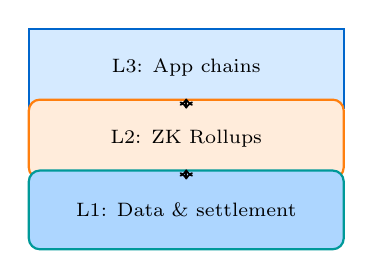
\begin{tikzpicture}[scale=0.6]
% Future stack
\node[process, minimum width=4cm, font=\scriptsize] (l3) at (0,3) {L3: App chains};
\node[l2box, minimum width=4cm, font=\scriptsize] (l2) at (0,1.5) {L2: ZK Rollups};
\node[l1box, minimum width=4cm, font=\scriptsize] (l1) at (0,0) {L1: Data \& settlement};

\draw[thick, <->] (l1) -- (l2);
\draw[thick, <->] (l2) -- (l3);
\end{tikzpicture}

\vspace{3mm}
\footnotesize Ethereum as ``settlement layer''\\
L2s for general compute\\
L3s for specific apps
\end{column}
\end{columns}
\end{frame}

% =======================================================================
% SLIDE 30: EXECUTIVE SUMMARY
% =======================================================================
\begin{frame}{Executive Summary: Key Takeaways}
\begin{enumerate}
\item \textbf{Layer 2 solves the scalability problem}\\
Process thousands of transactions off-chain, settle on L1 for security.

\vspace{2mm}
\item \textbf{Rollups are the dominant L2 approach}\\
Post all data to L1, enabling trustless verification and exits.

\vspace{2mm}
\item \textbf{Optimistic = assume valid, prove fraud}\\
7-day withdrawal, but mature and EVM-compatible.

\vspace{2mm}
\item \textbf{ZK = prove validity cryptographically}\\
Instant finality, but computationally expensive and newer.

\vspace{2mm}
\item \textbf{Bridges are critical infrastructure but high-risk}\\
\$1B+ lost to bridge hacks -- use with caution.

\vspace{2mm}
\item \textbf{L2s unlock mass adoption}\\
90\%+ fee reduction makes Ethereum usable for everyone.
\end{enumerate}
\end{frame}

% =======================================================================
% SLIDE 31: CONCEPT MAP
% =======================================================================
\begin{frame}{Concept Map: Layer 2 Ecosystem}
\begin{center}
\begin{tikzpicture}[scale=0.7, transform shape, node distance=1cm]
% Central L1
\node[l1box, minimum width=3cm] (l1) at (0,0) {\textbf{Ethereum L1}};

% L2 Solutions branching out
\node[l2box, minimum width=2.2cm, font=\small] (channels) at (-5,2) {Payment\\Channels};
\node[l2box, minimum width=2.2cm, font=\small] (sidechains) at (-2.5,3) {Sidechains};
\node[l2box, minimum width=2.2cm, font=\small] (optimistic) at (2.5,3) {Optimistic\\Rollups};
\node[l2box, minimum width=2.2cm, font=\small] (zk) at (5,2) {ZK\\Rollups};

% Examples
\node[databox, below=0.3cm of channels, font=\tiny] {Lightning};
\node[databox, below=0.3cm of sidechains, font=\tiny] {Polygon PoS};
\node[databox, below=0.3cm of optimistic, font=\tiny] {Arbitrum, Optimism};
\node[databox, below=0.3cm of zk, font=\tiny] {zkSync, StarkNet};

% Connections
\draw[thick, dfblue] (l1) -- (channels);
\draw[thick, dfblue] (l1) -- (sidechains);
\draw[thick, dfblue] (l1) -- (optimistic);
\draw[thick, dfblue] (l1) -- (zk);

% Properties box
\node[draw, thick, rounded corners, fill=dflightblue4, minimum width=8cm, text width=7.5cm, align=center, font=\scriptsize] at (0,-2.5) {
\textbf{All L2s share:} Lower fees | Higher throughput | Data to L1\\
\textbf{Key difference:} Trust model and finality speed
};

% Bridge
\node[bridgebox, minimum width=2cm, font=\tiny] at (0,1.5) {Bridges};
\end{tikzpicture}
\end{center}
\end{frame}

% =======================================================================
% SLIDE 32: KEY TERMS 1
% =======================================================================
\begin{frame}{Key Terms \& Definitions (1/2)}
\begin{description}
\item[Layer 2 (L2)] A secondary framework built on top of an existing blockchain (L1) to improve scalability while inheriting L1 security.

\item[Rollup] An L2 that executes transactions off-chain but posts transaction data to L1, enabling anyone to reconstruct the state.

\item[Optimistic Rollup] A rollup that assumes transactions are valid by default and uses fraud proofs to catch invalid state transitions.

\item[ZK-Rollup] A rollup that uses zero-knowledge proofs to cryptographically prove transaction validity, enabling instant finality.

\item[Data Availability] The guarantee that transaction data is published and accessible, allowing anyone to verify the L2 state.
\end{description}
\end{frame}

% =======================================================================
% SLIDE 33: KEY TERMS 2
% =======================================================================
\begin{frame}{Key Terms \& Definitions (2/2)}
\begin{description}
\item[Fraud Proof] A cryptographic proof submitted during a challenge period showing that a state transition was invalid.

\item[Validity Proof] A cryptographic proof (SNARK = Succinct Non-interactive ARgument of Knowledge / STARK = Scalable Transparent ARgument of Knowledge) that mathematically proves all transactions in a batch are valid.

\item[Sequencer] The entity responsible for ordering and batching L2 transactions before posting to L1.

\item[Bridge] A protocol enabling assets to move between different blockchains or layers by locking on one chain and minting on another.

\item[Payment Channel] An L2 mechanism allowing two parties to transact off-chain unlimited times, only settling on-chain when closing.
\end{description}
\end{frame}

% =======================================================================
% SLIDE 34: COMMON MISCONCEPTIONS
% =======================================================================
\begin{frame}{Common Misconceptions}
\begin{tabular}{p{4.8cm}|p{5.8cm}}
\textbf{Myth} & \textbf{Reality} \\
\hline
& \\
``L2s are less secure than L1'' & Rollups \textbf{inherit L1 security} because all data is on L1. Users can always exit to L1 if the L2 fails. \\[3mm]
\hline
& \\
``All L2s are the same'' & Different L2 types have \textbf{vastly different trust models}. Sidechains have independent security; rollups inherit L1 security. \\[3mm]
\hline
& \\
``7-day withdrawal means 7 days to use funds'' & The 7-day challenge period is only for \textbf{L2$\rightarrow$L1 withdrawals}. On L2, transactions are instant. This delay exists to give anyone time to challenge potentially fraudulent transactions. \\[3mm]
\hline
& \\
``ZK-rollups are always better'' & ZK-rollups have \textbf{tradeoffs}: higher proving costs, developing EVM compatibility, and newer technology. \\
\end{tabular}
\end{frame}

% =======================================================================
% SLIDE 35: SELF-ASSESSMENT 1
% =======================================================================
\begin{frame}{Self-Assessment Questions (1/2)}
\textbf{Question 1:} What is the main difference between Optimistic and ZK-Rollups?

\vspace{2mm}
\begin{enumerate}[A.]
\item Optimistic rollups are faster than ZK-rollups
\item Optimistic rollups use fraud proofs; ZK-rollups use validity proofs
\item ZK-rollups have a 7-day withdrawal period
\item Optimistic rollups don't post data to L1
\end{enumerate}

\vspace{5mm}
\pause
\textcolor{dfgreen}{\textbf{Answer: B}}

\textit{Explanation:} Optimistic rollups assume validity and only compute proofs if challenged (fraud proofs). ZK-rollups prove validity cryptographically before posting (validity proofs). This is why ZK-rollups have instant finality while optimistic rollups need a 7-day challenge period (to give anyone time to challenge potentially fraudulent transactions).
\end{frame}

% =======================================================================
% SLIDE 36: SELF-ASSESSMENT 2
% =======================================================================
\begin{frame}{Self-Assessment Questions (2/2)}
\textbf{Question 2:} Why are bridges considered high-risk infrastructure?

\vspace{2mm}
\begin{enumerate}[A.]
\item Bridges are slower than direct L1 transactions
\item Bridges hold large amounts of locked assets and have complex smart contracts
\item Bridges don't support all tokens
\item Bridges are not decentralized
\end{enumerate}

\vspace{3mm}
\pause
\textcolor{dfgreen}{\textbf{Answer: B}}

\textit{Explanation:} Bridges are attractive targets because they hold large TVL, have complex cross-chain logic, and often rely on centralized components. Over \$1B has been lost to bridge hacks (Ronin, Wormhole, Nomad).

\vspace{3mm}
\textbf{Question 3:} What makes rollup security different from sidechain security?

\pause
\textcolor{dfgreen}{\textbf{Answer:}} Rollups post all transaction data to L1, inheriting L1 security. Sidechains have independent validators and their own security -- if sidechain validators collude, funds could be at risk.
\end{frame}

% =======================================================================
% SLIDE 37: WHAT'S NEXT
% =======================================================================
\begin{frame}{What's Next: Topic 4.1 -- Smart Contracts}
\textbf{From scaling to programming: How to build on blockchains}

\vspace{5mm}
\begin{columns}[T]
\begin{column}{0.48\textwidth}
\textbf{Topics we'll cover:}
\begin{itemize}
\item What is a smart contract?
\item Solidity programming basics
\item EVM execution model
\item Common patterns and pitfalls
\item Security considerations
\end{itemize}
\end{column}
\begin{column}{0.48\textwidth}
\textbf{Key insight preview:}
\begin{center}
\fbox{\parbox{0.9\textwidth}{
\textbf{Smart Contracts:}\\[2mm]
Code that executes exactly as written, with no human interpretation.\\[1mm]
``Code is law'' -- for better and worse.
}}
\end{center}
\end{column}
\end{columns}

\vspace{5mm}
\textbf{Connection to L2:} Most L2s are EVM-compatible, meaning smart contracts written for Ethereum can deploy to L2s with minimal changes -- same code, lower fees.
\end{frame}

% =======================================================================
% SLIDE 38: RESOURCES
% =======================================================================
\begin{frame}{Resources for Further Learning}
\textbf{Essential Reading:}
\begin{itemize}
\item Vitalik Buterin: ``An Incomplete Guide to Rollups'' (2021)
\item L2Beat: \url{https://l2beat.com} -- L2 risk analysis and metrics
\item Ethereum.org: Layer 2 documentation
\end{itemize}

\vspace{3mm}
\textbf{Data \& Analytics:}
\begin{itemize}
\item \textbf{L2Beat:} Comprehensive L2 comparison and risk assessment
\item \textbf{Arbiscan:} Arbitrum block explorer
\item \textbf{Optimistic Etherscan:} Optimism block explorer
\item \textbf{Dune Analytics:} L2 adoption dashboards
\end{itemize}

\vspace{3mm}
\textbf{Deep Dives:}
\begin{itemize}
\item Matter Labs blog: ZK-rollup technology explained
\item Paradigm research: Optimistic rollup design
\item StarkWare blog: STARKs vs. SNARKs
\end{itemize}

\bottomnote{NB15 provides hands-on exploration of L2 data and metrics}
\end{frame}

% =======================================================================
% SLIDE 39: QUESTIONS
% =======================================================================
\begin{frame}[plain]
\vfill
\begin{center}
{\Huge \textbf{Questions?}}

\vspace{10mm}
{\large Topic 3.5: Layer 2 Scaling Solutions [ADVANCED]}

\vspace{5mm}
{\normalsize Scaling Ethereum and Beyond}

\vspace{10mm}
\begin{tikzpicture}[scale=0.7]
% Simple L2 stack
\node[l2box, minimum width=6cm, minimum height=0.8cm] (l2) at (0,1) {\footnotesize Layer 2: Fast, Cheap};
\node[l1box, minimum width=6cm, minimum height=0.8cm] (l1) at (0,0) {\footnotesize Layer 1: Secure, Decentralized};
\draw[very thick, dfpurple, <->] (-2,0.4) -- (-2,0.6);
\draw[very thick, dfpurple, <->] (2,0.4) -- (2,0.6);
\end{tikzpicture}

\vspace{10mm}
\textcolor{dfblue}{\textbf{Next:} Topic 4.1 -- Smart Contracts}
\end{center}
\vfill
\end{frame}

% =======================================================================
% SLIDE 40: L2 COMPARISON REFERENCE
% =======================================================================
\begin{frame}{Reference: L2 Solutions Comparison}
\begin{center}
\begin{adjustbox}{max width=\textwidth}
\begin{tabular}{l|c|c|c|c|c}
\toprule
\textbf{Solution} & \textbf{Type} & \textbf{Security} & \textbf{Finality} & \textbf{TPS} & \textbf{EVM} \\
\midrule
Arbitrum One & Optimistic & L1 inherited & 7 days & 4,000+ & Yes \\
Optimism & Optimistic & L1 inherited & 7 days & 2,000+ & Yes \\
zkSync Era & ZK & L1 inherited & Minutes & 2,000+ & Yes \\
StarkNet & ZK & L1 inherited & Minutes & 1,000+ & No (Cairo) \\
Polygon PoS & Sidechain & Independent & Seconds & 7,000+ & Yes \\
Lightning & Channel & L1 inherited & Instant & 1M+ & No \\
\bottomrule
\end{tabular}
\end{adjustbox}
\end{center}

\vspace{3mm}
\textbf{2024 TVL Rankings:}
\begin{enumerate}\compactlist
\item Arbitrum: \$2.5B+
\item Optimism: \$800M+
\item Polygon: \$1B+ (sidechain)
\item zkSync: \$150M+
\item StarkNet: \$200M+
\end{enumerate}

\vspace{3mm}
\footnotesize Source: L2Beat, DeFiLlama (data as of 2024)
\end{frame}

\end{document}
